\chapter{Analyse}

\section{Augmented Reality Frameworks}

%ARKit ARCore SLAM!

%Vuforia, Wikitude... Marker, Natural Feature, 3dObject

%Visionlib 3D Objekt spezialisiert. 

%Unterschide 3D Objekt basiert Vuforia und visionlib: Vuforia - keine Objekte mit geringer geometrischen eigenschaften. Vuforia, bewegungsempfindlich. 

%Vuforia kann mit ARCore oder ARKit kombiniert werden!

\section{Annotationen in AR}

\cite{Brandenburg2019}

\section{Zeigen und Auswählen in AR Benutzeroberflächen}

In diesem Abschnitt werden Grundlagen für das zeigen und Auswählen in Virtuellen Umgebungen behandelt, sowie einige aktuelle Arbeiten 
zu diesem Thema näher betrachtet. 

Der digitale Prototyp soll auf Android Smartphone mit einer Touchscreen Bildschirmoberfläche implementiert werden.
\cite[S.~205]{Ortega2016} beschreit folgende grundsätzliche Probleme welche bei Interaktionen auf diesen Oberflächen auftreten können und daher beachtet werden sollten:  
Dadurch dass Interaktionen mit dem direkten Berühren des Bildschirmes stattfinden fehlt bei Touch Oberflächen das Drüber schweben (engl. Hover) bevor eine Aktion durch das Klicken der Maus Taste bestätigt wird. 
Dadurch dass der Finger auf den Bildschirm aufgelegt wird, besteht das Problem der Verdeckung. Zudem muss mit stark variierender Sinn für Präzision gerechnet werden. \cite[S.~205]{Ortega2016} ordnet Ansätze 
für den Behandlung mit diesen Probleme in zwei Gruppen: 


Hauptprobleme: - kein Hover -Überdeckung (Occulusion) - Prezision -Fehlen oder nicht adäquater visueller Rückmeldung. 
Größe des Fingers und stark variierende Sinn für Präzision erschweren Gestaltung für Interaktionen auf Touch Bildschirmen.

Zwei Ansätze: 1) Das Präzise Auswählen wird an die Gestaltung der Benutzeroberfläche übergeben. Deshalb präziser Auswahl wird als neue Anforderung 
an die Oberfläche übertragen. 2) 

Diese Probleme machen Touchscreen Oberflächen schwierig für preise Interaktionen  


\cite[S.~150]{Bowman2011}
% Andeuten 
% Bestätigen
% Rückmeldung

%Bowman: At close range, ray-casting is a simple and eficcient selection technique

\begin{figure}[H]
	\centering
	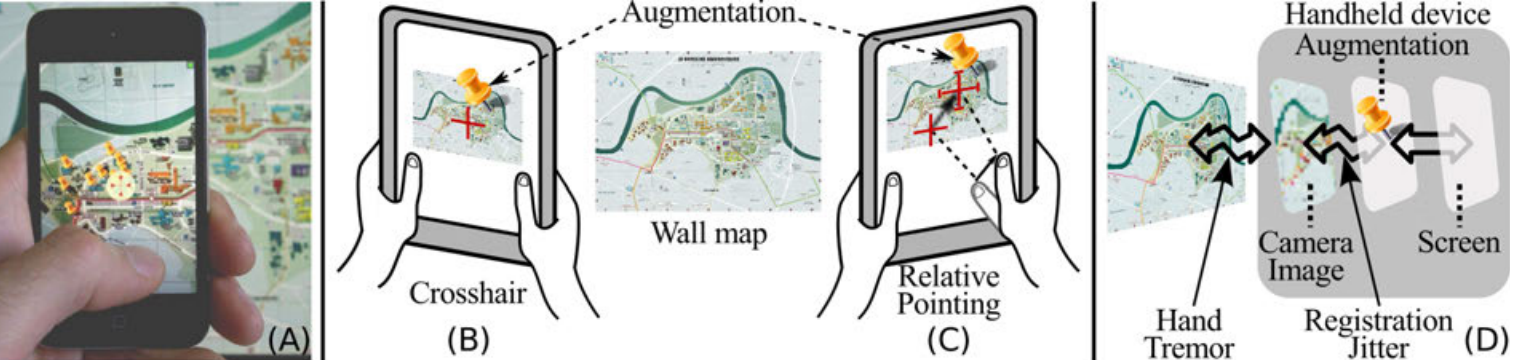
\includegraphics[width=1.0\textwidth]{resources/analyse/Pointing_techniken.png}
	\caption{Online-Produktkommentierung über Listen- und Bildzugang. Quelle: \cite{Vincent2013}}
	\label{img:pointing_vergleich}
\end{figure}

\begin{figure}[H]
	\centering
	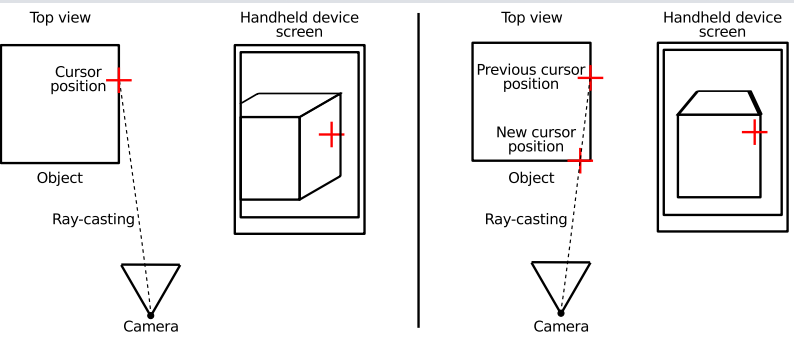
\includegraphics[width=1.0\textwidth]{resources/analyse/pointing_3d.png}
	\caption{Relative Pointing auf der Oberfläche von 3D Objekten. Quelle: \cite[S.~92]{Vincent2014}}
	\label{img:pointing_vergleich}
\end{figure}

\section{Kundenintegration}

%Definition und Grobkonzept

\begin{figure}[H]
	\centering
	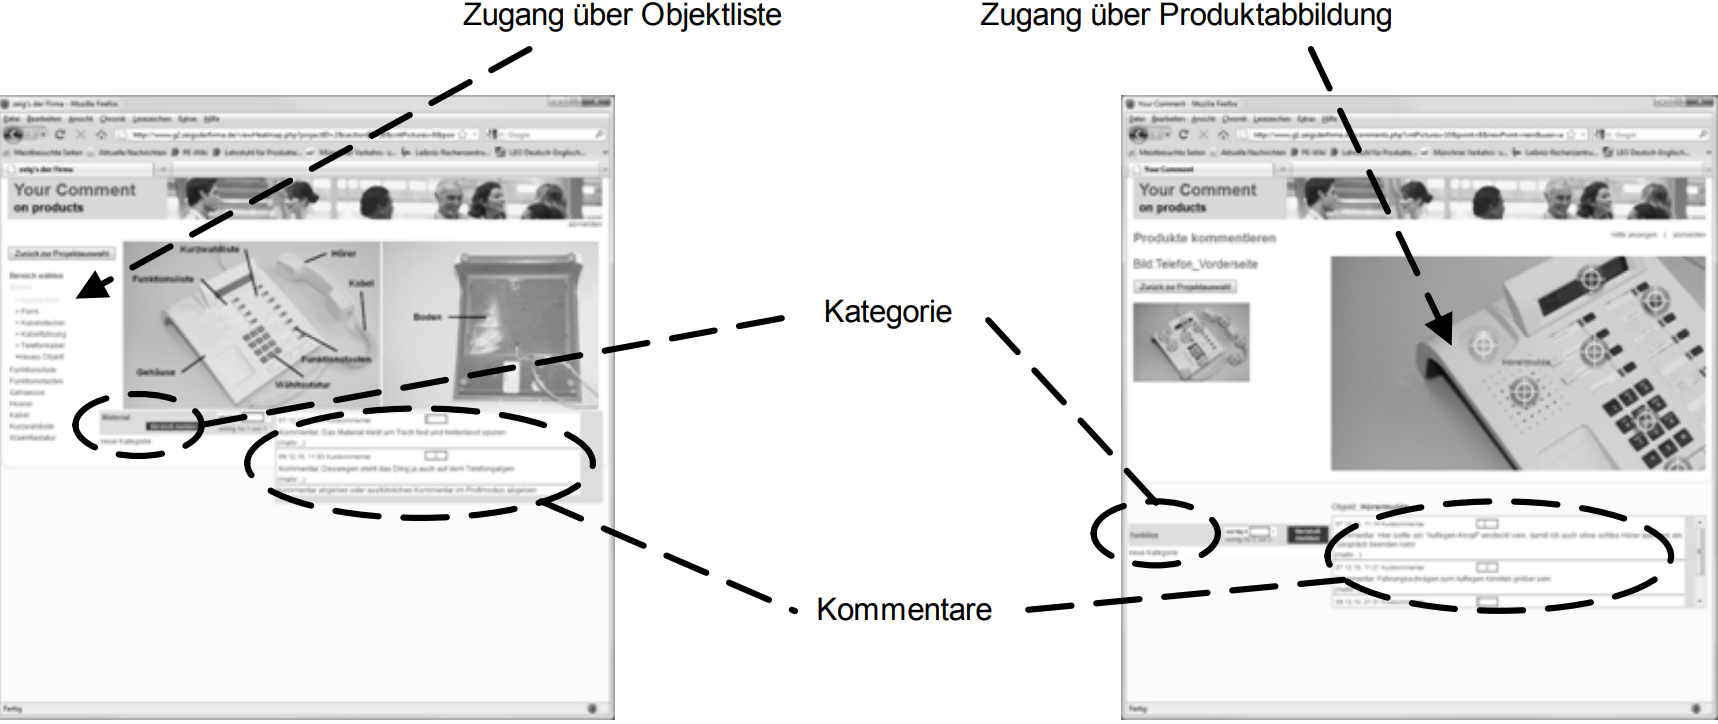
\includegraphics[width=1.0\textwidth]{resources/analyse/IPI_Vergleich_Listen_BildAnnotationeAnsicht.png}
	\caption{Online-Produktkommentierung über Listen- und Bildzugang. Quelle: \cite[S.~7]{Kirschner2011}}
	\label{img:ipi_list_image}
\end{figure}

\begin{figure}[H]
	\centering
	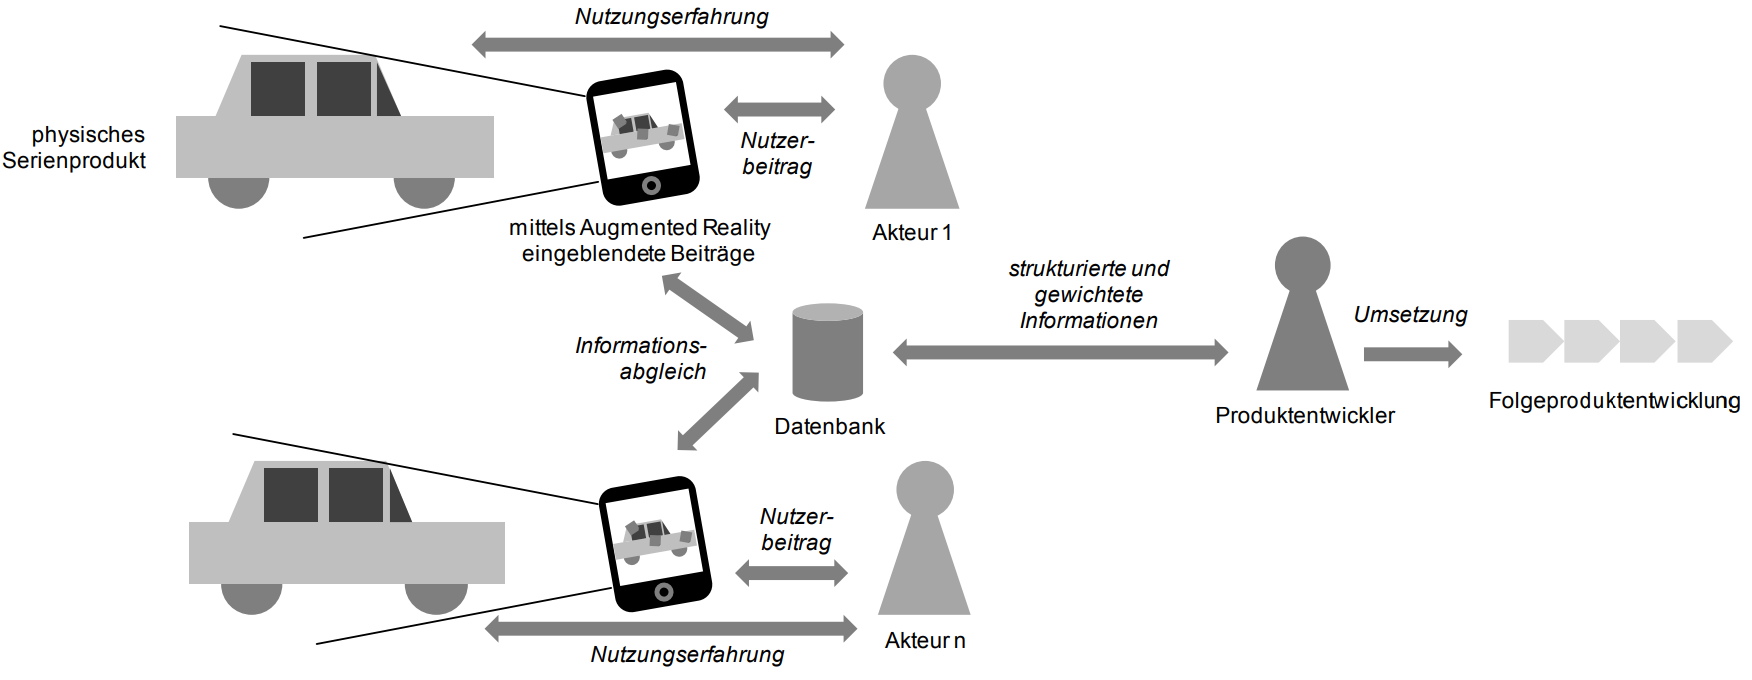
\includegraphics[width=1.0\textwidth]{resources/analyse/IPI_Objektzentriert.png}
	\caption{Informationsfluss  in der objektzentrierten IPI-Umsetzung. Quelle:\cite[S.~135]{Kirschner2012}}
	\label{img:objekt_centered_ipi}
\end{figure}


%kurz pysische 

%Bildzentriert. Vergleich mit Liste. Ergebnisse der Studie aus 2011

% Objektzentriert.

\section{Zusammenfassung}